\documentclass{article}
\usepackage{graphicx} % Required for inserting images
\usepackage{varwidth}
\usepackage{xcolor}
\usepackage{listings}


\definecolor{codegreen}{rgb}{0,0.6,0}
\definecolor{codegray}{rgb}{0.5,0.5,0.5}
\definecolor{codepurple}{rgb}{0.58,0,0.82}
\definecolor{backcolour}{rgb}{0.95,0.95,0.92}

\lstdefinestyle{CStyle}{
	language=C++,
	backgroundcolor=\color{backcolour},   
	commentstyle=\color{codegreen},
	keywordstyle=\color{magenta},
	numberstyle=\tiny\color{codegray},
	stringstyle=\color{codepurple},
	basicstyle=\ttfamily\footnotesize,
	breakatwhitespace=false,         
	breaklines=true,                 
	keepspaces=true,                 
	numbers=left,       
	numbersep=5pt,                  
	showspaces=false,                
	showstringspaces=false,
	showtabs=false,                  
	tabsize=2,
}
\lstset{style=CStyle}

\title{Lab 3 Report \\ \large EEL4742C - 00446}
\author{Yousef Awad}
\date{September 2025}
\setcounter{secnumdepth}{0}

\begin{document}

\maketitle
\tableofcontents
\newpage

\section{Introduction}
I don't have time for this, sorry :(

\section{3.1 Continuous Mode}
The continuous mode here causes the timer to just count from 0 to 65,535. This, therefore, means that there will be 65,536 of counted cycles before the flag is raised. Knowing this, with the addition that there is 32,768 cycles per second, we therefore know that the amount of time for per switching red led will be $\frac{65,536}{32,768} = 2\ seconds$. This was then validated via my phone's stopwatch and after 10 cycles, all came to an average of 2 seconds per switch. If we set the input divider to say 2, or 4, or 8, then it would expand the delay to 4, 8, or 16 seconds respectively per switch on and off.
\begin{lstlisting}
#include <msp430.h>

#define redLED BIT0
#define greenLED BIT7

// Configures ACLK to 32 KHz crystal
void config_ACLK_to_32KHz_crystal() 
{
  // By default, ACLK runs on LFMODCLK at 5MHz/128 = 39 KHz
  // Reroute pins to LFXIN/LFXOUT functionality
  PJSEL1 &= ~BIT4;
  PJSEL0 |= BIT4;
  // Wait until the oscillator fault flags remain cleared
  CSCTL0 = CSKEY; // Unlock CS registers
  do 
	{
    CSCTL5 &= ~LFXTOFFG; // Local fault flag
    SFRIFG1 &= ~OFIFG;   // Global fault flag
  } while ((CSCTL5 & LFXTOFFG) != 0);
  CSCTL0_H = 0; // Lock CS registers
  return;
}

int main(void)
{
  WDTCTL = WDTPW | WDTHOLD; // Stop the Watchdog timer
  PM5CTL0 &= ~LOCKLPM5;     // Disable GPIO power-on default high-impedance mode
  // assign redLED and greenLED outputs
  P1DIR |= redLED;
  P9DIR |= greenLED;
  // turn off LEDs by default
  P1OUT &= ~redLED;
  P9OUT &= ~greenLED;
  // calling function to configure ACLK
  config_ACLK_to_32KHz_crystal();
  // configure Timer_A
  // use ACLK, divide by 1, continuous mode, clear TAR
  TA0CTL = TASSEL_1 | ID_3 | MC_2 | TACLR;
  // Changing ID_0 will make the timer longer
  // ensure flag is cleared before running infinite for loop
  TA0CTL &= ~TAIFG;
  for (;;)
	{
    while ((TA0CTL & TAIFG) != TAIFG)
		{
    }; // delay until flag is set
    P1OUT ^= redLED;  // toggle LED
    TA0CTL &= ~TAIFG; // reset flag
  } // end infinite for loop
} 
\end{lstlisting}

\section{3.2 Up Mode}
To set the timer cycle to one second, and then have it simply turn switch the red led we would need to know the amount of cycles that occur in a second, of which for the msp430 clock we've set it too is 32KHz or 32,768 cycles. To change the amount of time per switch we simply need to divide by 10 to the cycle count for 0.1 second or 100 for 0.01 seconds.
\begin{lstlisting}
#include <msp430.h>
#define redLED BIT0
#define greenLED BIT7

// Configures ACLK to 32 KHz crystal
void config_ACLK_to_32KHz_crystal() 
{
  // By default, ACLK runs on LFMODCLK at 5MHz/128 = 39 KHz
  // Reroute pins to LFXIN/LFXOUT functionality
  PJSEL1 &= ~BIT4;
  PJSEL0 |= BIT4;
  // Wait until the oscillator fault flags remain cleared
  CSCTL0 = CSKEY; // Unlock CS registers
  do
	{
    CSCTL5 &= ~LFXTOFFG; // Local fault flag
    SFRIFG1 &= ~OFIFG;   // Global fault flag
  } while ((CSCTL5 & LFXTOFFG) != 0);
  CSCTL0_H = 0; // Lock CS registers
  return;
}

int main(void)
{
  WDTCTL = WDTPW | WDTHOLD; // Stop the Watchdog timer
  PM5CTL0 &= ~LOCKLPM5;     // Disable GPIO power-on default high-impedance mode
  // assign redLED and greenLED outputs
  P1DIR |= redLED;
  P9DIR |= greenLED;
  // turn off LEDs by default
  P1OUT &= ~redLED;
  P9OUT &= ~greenLED;
  // calling function to configure ACLK
  config_ACLK_to_32KHz_crystal();
  // configure Timer_A
  // use ACLK, divide by 1, Up mode, clear TAR
  TA0CTL = TASSEL_1 | ID_0 | MC_1 | TACLR;
  // TA0CCR0 = 327.67; //0.01s delay
  // TA0CCR0 = 3276.7; //0.1s delay
  TA0CCR0 = 32767; // 1s delay

  // ensure flag is cleared before running infinite for loop
  TA0CTL &= ~TAIFG;
  for (;;)
	{
    while ((TA0CTL & TAIFG) != TAIFG) 
		{
    }; // delay until flag is set
    P1OUT ^= redLED;  // toggle LED
    TA0CTL &= ~TAIFG; // reset flag
  } // end infinite for loop
} // end main
\end{lstlisting}

\section{3.3 Signal Repeater}
The maximum delay for all divider cases is as follows:
\begin{itemize}
	\item ID\_0: $$ \frac{1}{32,768}\ sec/cycles=3.052\ microsec * 65,536 cycles = 2\ seconds$$
	\item ID\_1: $$ \frac{1}{32,768/2}\ sec/cycles=6.103\ microsec * 65,536 cycles = 4\ seconds$$
	\item ID\_2: $$ \frac{1}{32,768/4}\ sec/cycles=12.207\ microsec * 65,536 cycles = 8\ seconds$$
	\item ID\_3: $$ \frac{1}{32,768/8}\ sec/cycles=24.414\ microsec * 65,536 cycles = 16\ seconds$$
\end{itemize}
The specific tradeoff between dividers is that a lower dividers allows for more specific and accurate measurements of how much time has passed (or at least cycles). A higher divider, though, does allow for us to measure larger amounts of time.
\newline
The code can be modified, with how I have it we simply need to keep track of the amount of overflows that occur in a given amount of time and would therefore allow for, at least, 65,536 overflows to occur, and then use that to calculate the exact amount of time that has progressed.
\begin{lstlisting}
#include <inttypes.h>
#include <msp430.h>
#define redLED BIT0
#define greenLED BIT7
#define but1 BIT1
#define but2 BIT2

//**********************************
// Configures ACLK to 32 KHz crystal
void config_ACLK_to_32KHz_crystal() {
  // By default, ACLK runs on LFMODCLK at 5MHz/128 = 39 KHz
  // Reroute pins to LFXIN/LFXOUT functionality
  PJSEL1 &= ~BIT4;
  PJSEL0 |= BIT4;
  // Wait until the oscillator fault flags remain cleared
  CSCTL0 = CSKEY; // Unlock CS registers
  do {
    CSCTL5 &= ~LFXTOFFG; // Local fault flag
    SFRIFG1 &= ~OFIFG;   // Global fault flag
  } while ((CSCTL5 & LFXTOFFG) != 0);
  CSCTL0_H = 0; // Lock CS registers
  return;
}

int main(void) {
  WDTCTL = WDTPW | WDTHOLD; // stop watchdog timer
  PM5CTL0 &= ~LOCKLPM5;     // opening gpio

	// setting direction to inputs and outputs of red, green, and buttons
  P1DIR |= redLED;
  P9DIR |= greenLED;
  P1DIR &= ~(but1 | but2);

	// Setting green led as outputs
  P1OUT &= ~redLED;
  P9OUT &= ~greenLED;
  P1OUT |= but1 | but2;

	// Setting resistor
  P1REN |= but1 | but2;

	// Setting the clock
  config_ACLK_to_32KHz_crystal();

  for (;;) {
    while ((P1IN & but1) != 0) 
		{
			// While but1 is pressed, do nothing lmao
    }
    TA0CTL = TASSEL_1 | ID_0 | MC_2 | TACLR; // setting the clock thing to continiuous.
    TA0CTL &= ~TAIFG; // AND with inverse of mask to clear the bit
    while (((P1IN & but1) == 0) && (TA0CTL & TAIFG) == 0) 
		{
			// button1 is not pressed and no overflow occured, loop and do nthing
    }
    if ((TA0CTL & TAIFG) != 0)
		{
			// overflo of timer occured
      P9OUT |= greenLED; // turn on green led.
      while ((P1IN & but2) != 0)
			{
				// while the button2 not pressed, wait
      }
			// button2 was pressed therefore clear green led and reset timer
      P9OUT &= ~greenLED;
      TA0CTL &= ~TAIFG; // AND with inverse of mask to clear the bit
    } 
	  else
		{
			// overflow did not occur therefore flash green led correct time
      TA0CCR0 = TA0R;
      TA0CTL = TASSEL_1 | ID_0 | MC_1 | TACLR; // timer now using up mode with end time = time
      TA0CTL &= ~TAIFG; // AND with inverse of mask to clear the bit
											
      P1OUT |= redLED;
      while ((TA0CTL & TAIFG) == 0) 
			{
      }
      TA0CTL &= ~TAIFG; // AND with inverse of mask to clear the bit
      P1OUT &= ~redLED;
    }
    TA0CTL &= ~TAIFG; // AND with inverse of mask to clear the bit
    TA0CTL = MC_0 | TACLR;
  }
}
\end{lstlisting}

\section{Student Q\&A}
\subsection{1}
Using Timer\_A is more accurate and gives you more control when compared to the delay loop. This is due to the fact that the timer is independant of the CPU in its entirety and is therefore only controlled by the embedded programmer, and only is dependant on the clock. 

\subsection{2}
The polling technique is simply the CPU checking whether or not a flag has been set (aka TAIFG or CCIFG or whatever). One cycle after that flag is set, the CPU then realizes it and acts upon the conditions that are reliant on the flag going up.

\subsection{3}
If we wanted to save battery power, the constant polling technique we are using above is \textit{not} the one that we should use. Instead we should a low power mode that doesn't check every cycle whether or not the flog is raised.

\subsection{4}
No, setting the TAR to 0 via software will only reset the timer's counter, BUT NOT set the TAIFG flag to 1. TAIFG only raises when the counter overflows.

\subsection{5}
The UP Mode gives more control over timing duration due to us having the ability to set when a flag (other than TAIFG) is raised instead of continuous which only raises when the counter overflows.

\subsection{6}
Here is the documentation on the Timer\_A layout.
\newline
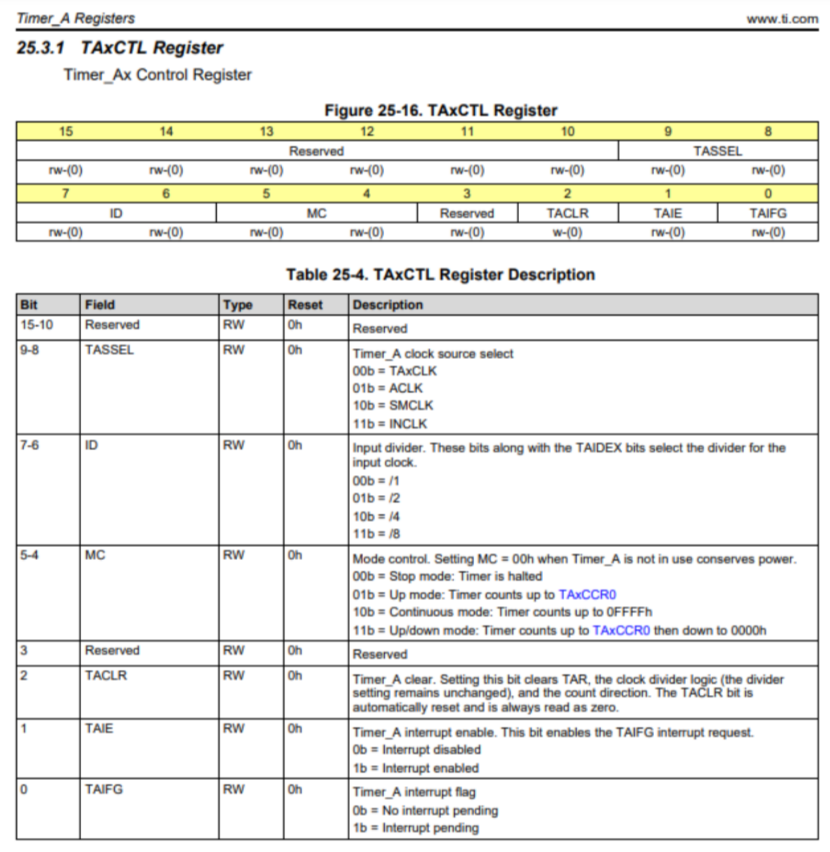
\includegraphics[width=1\textwidth]{pictures/image.png}


\end{document}
